% don't remove the folling lines, and edit the defintion of \main if needed
\documentclass[../report.tex]{subfiles}
\providecommand{\main}{..}
\IfEq{\jobname}{\currfilebase}{\AtEndDocument{\biblio}}{}
% until here

\begin{document}

\section{Searches for beyond the standard model Higgs physics}

\emph{Make sure your contribution is in a separate file!}

\subfile{\main/section9/mssm_2hdm}

\subsection{Production of $t\bar{t}h$ and $t\bar{t}h h$ at the LHC in Composite Higgs models}
\subfile{\main/section9/MCHM_tthh}

\subsection{Exotic decays of the Higgs boson}
\subfile{\main/section9/h4jet}
\subfile{\main/section9/summary_of_2b2mu}
\subfile{\main/section9/HiggsToALPs}

\subsection{Searches for additional Higgs bosons in fermionic final states}
\subfile{\main/section9/cms_htt/mssm_cms}
\subfile{\main/section9/atlas_htautau/mssmtautau}
\subfile{\main/section9/lhcb_amumu/lhcb}

\subsection{Searches for additional Higgs bosons in diboson final states}


\subsection{MSSM charged Higgs bosons}
\subfile{\main/section9/MSSMCharged}

\clearpage

\vspace{5cm}
\subsection{All contributions below: Move your contribution to a separate file!}




\subsection{Interpretation of the Higgs couplings in terms of Composite Higgs models}
\label{sec9:CHM}
\begin{center}
 {L. Vecchi\\
}
%\noindent
 {\small Theoretical Particle Physics Laboratory, Institute of Physics, EPFL, Lausanne, Switzerland}
\end{center}

\subsubsection{Introduction}

\begin{itemize}
\item Composite Higgs (CH) models provide a natural solution to the hierarchy problem. Main assumption: a strong sector generates a light scalar $H$ (with the same charges of the SM Higgs doublet) that breaks $SU(2)\times U(1)$. %The latter may or may not be a Nambu-Goldstone mode. If it is, then it is also naturally weakly-coupled and lighter than all other resonances. If it is not, additional tunings are needed.

\item Several realizations of the CH proposed in the literature predict the existence of additional light particles beyond the Higgs, e.g. scalars in non-minimal $G\to H$, a dilaton in nearly-conformal models, fermion resonances to reduce the fine-tuning, vector resonances in Little Higgs models. Here however we will assume that all exotic particles are heavy enough to be directly inaccessible. Within this assumption, an effective field theory formalism becomes reliable.


\item The main goal of this section is to (1) review what are the most important corrections to the Higgs couplings that are expected if the Higgs is a composite state; (2) estimate the sensitivity of the HL and HE-LHC on the CH picture. We will focus on modifications of the Higgs couplings (as opposed to off-shell rates like double-Higgs production or $VV\to VV,hh$ scattering). 


\item Up to dimension 6, the operators that can potentially impact on-shell processes involving the Higgs boson are collected in table \ref{tab1}. Note that ${O}_r=H^\dagger H(D_\mu H)^\dagger D^\mu H$ is not part of the set because equivalent to a linear combination of $\sum_\psi{\cal O}_\psi$ and ${\cal O}_{H,6}$. Similarly, $gg'H^\dagger\sigma^i HW^i_{\mu\nu}B^{\mu\nu}$ and $g^2H^\dagger HW^i_{\mu\nu}W^{i\mu\nu}$, as well as their CP-odd versions, are not independent. Finally, there is a set of operators involving the Higgs doublet that are severely constrained by precision data, and for this reason are expected to be negligible in our analysis. These include $O_T=\frac{1}{2}~(H^\dagger\overleftrightarrow{D_\mu}H)(H^\dagger\overleftrightarrow{D^\mu}H)$, current-current interactions $H^\dagger \overleftrightarrow{D^\mu}H \bar \psi\gamma^\mu \psi$ and $H^\dagger \tau^a\overleftrightarrow{D^\mu}H \bar \psi\gamma^\mu \tau^a\psi$ containing non-universal couplings to the SM fermions $\psi$, and dipole operators. The coefficient of the operator $O_T$ contributes to the EW $T$ parameter, and may be suppressed assuming the strong sector respects a custodial $SU(2)$ symmetry. The current-current operators are constrained by LEP and the non-observation of rare flavor-violating processes. Dipole operators are severely constrained by measurements of dipole moments. (The only exception is provided by those interactions involving the top...)




\end{itemize}




%%%%%%%%%%%%%%%%%%%%%
\begin{table}[t]
\begin{center}
%\resizebox{\textwidth}{!}
{
\begin{tabular}{c|c||c|c} 
\rule{0pt}{1.2em}%
Operator name & Operator definition & Main On-shell (Higgs) \\
\hline
${\cal O}_H$ & $\frac{1}{2}~\partial_\mu(H^\dagger H)\partial^\mu(H^\dagger H)$ & $h\to\psi\bar\psi, VV^*$     \\
${\cal O}_T$ & $\frac{1}{2}~(H^\dagger\overleftrightarrow{D_\mu}H)(H^\dagger\overleftrightarrow{D^\mu}H)$ & $h\to ZZ^*$  \\
${\cal O}_6$ & $\lambda_h(H^\dagger H)^3$ & ${\rm off-shell}~h^*\leftrightarrow hh$  \\
${\cal O}_\psi$ & $y_\psi~\overline\psi_L H\psi_R(H^\dagger H)$ & $h\to\psi\bar\psi$  \\
\hline
${\cal O}_W$ & $\frac{i}{2}~g(H^\dagger\sigma^i\overleftrightarrow{D_\mu} H)(D_\nu W^{\mu\nu})^i$ & $h\to VV^*$ \\
${\cal O}_B$ & $\frac{i}{2}~g'(H^\dagger\overleftrightarrow{D_\mu} H)(\partial_\nu B^{\mu\nu})$ & $h\to VV^*$  \\
%
${\cal O}_{HW}$ & $ig(D^\mu H)^\dagger\sigma^i(D^\nu H)W_{\mu\nu}^i$ & $h\to VV^*,\gamma Z$  \\
${\cal O}_{HB}$ & $ig'(D^\mu H)^\dagger(D^\nu H)B_{\mu\nu}$ & $h\to VV^*,\gamma Z$ \\
\hline
${\cal O}_{g}$ & $g_s^2H^\dagger H G^a_{\mu\nu}G^{a\mu\nu}$ & $h\to gg$  \\
${\cal O}_{\gamma}$ & $g'^2H^\dagger HB_{\mu\nu}B^{\mu\nu}$ & $h\to \gamma\gamma,\gamma Z^0,Z^0Z^0$ 
%
\end{tabular}
}
\end{center}
\caption{\small List of the most relevant dimension-6 operators in the study of modified Higgs couplings in CH models. We use the basis of~\cite{Giudice:2007fh}. Here $y_\psi$ are the SM Yukawa couplings and $V=Z^0,W^\pm$. CP-odd versions of ${HW,HB,\gamma,g}$ can be obtained by replacing one field strength with the corresponding dual, $F^{\mu\nu}\to\frac{1}{2}\epsilon^{\mu\nu\alpha\beta}F_{\alpha\beta}$. The third column shows the dominant on-shell Higgs processes that the operator contributes to. 
\label{tab1}}
\end{table}
%%%%%%%%%%%%%%%%%%%%%%%





\subsubsection{Modified Higgs couplings}

\begin{itemize}
\item The observables that are mostly affected by the new operators are shown in the third column of table \ref{tab1}. An estimate of the various Wilson coefficients in concrete CH models reveals that (1) corrections to $h\to VV^*$ are typically dominated by ${\cal O}_{H,\psi}$, (2) corrections to the radiative processes $h\to gg,\gamma\gamma,Z^0\gamma$ are controlled by ${\cal O}_{H,\psi}$ if the Higgs is a Nambu-Goldstone mode and receive important contributions also from ${\cal O}_{g,\gamma}$ if $H$ is an accidentally resonance. The bottom line is that the reduced set of operators 
\begin{eqnarray}\label{SMEFT}
\delta{\cal L}_{\rm eff}=\frac{g_*^2}{m_*^2}c_H{\cal O}_H+\frac{g_*^2}{m_*^2}\sum_\psi c_\psi{\cal O}_\psi+\frac{1}{m_*^2}c_g{\cal O}_g+\frac{1}{m_*^2}c_\gamma{\cal O}_\gamma,
\end{eqnarray}
can be used to characterize the most common signatures of realistic CH models.
\item A few benchmark models in which the coefficients can be reliably estimated is presented. For example, a $O(5)/O(4)$ CH model with fermions in some representation of $O(5)$. The possible existence of additional symmetries (custodial symmetry, $G\to H$, $T$-parity, etc.) has implicatios on the Wilson coefficients.

\item We can now match the Wilson coefficients derived above onto a Lagrangian for the physical Higgs (see e.g. \cite{Contino:2013kra}):
\begin{eqnarray}\label{Lh}
{\cal L}_h&=&\frac{1}{2}\partial_\mu h\partial^\mu h-\frac{1}{2}m_h^2h^2\\\nonumber
&+&\left[m_W^2W^+_\mu W^{-\mu}+\frac{1}{2}m_Z^2Z_\mu Z^\mu\right]\left(1+c_V\frac{h}{v}+\cdots\right)\\\nonumber
&-&\sum_{\psi=u,d,l}m_\psi\bar\psi\psi\left(1+c_\psi\frac{h}{v}+\cdots\right)\\\nonumber
&+&\left[\frac{1}{2}c_{gg}G^a_{\mu\nu}G^{a\mu\nu}+\frac{1}{2}c_{\gamma\gamma}\gamma_{\mu\nu}\gamma^{\mu\nu}+\frac{1}{2}c_{ZZ}Z_{\mu\nu}Z^{\mu\nu}+c_{Z\gamma}Z_{\mu\nu}\gamma^{\mu\nu}\right]\frac{h}{v}\\\nonumber
&+&\cdots
\end{eqnarray}
with the modified Higgs couplings defined by
\begin{eqnarray}\label{cs}
c_V&=&1-\frac{c_H}{2}\xi\\\nonumber
c_\psi&=&1-\left(\frac{c_H}{2}+c_\psi\right)\xi\\\nonumber
c_{gg}&=&2\frac{g_s^2}{g_*^2}\xi c_g\\\nonumber
c_{\gamma\gamma}=-\frac{c_{Z\gamma}}{\tan\theta_W}=\frac{c_{ZZ}}{\tan^2\theta_W}&=&2\frac{e^2}{g_*^2}\xi c_\gamma
\end{eqnarray}
and
\begin{eqnarray}
\xi\equiv\frac{g_*^2v^2}{m_*^2}.
\end{eqnarray}
\item We can then present the expected reach of the HL and HE LHC on the modified Higgs couplings. {\color{red} This is where some experimental input would be appreciated.} We can briefly compare it with current constraints and proposed experiments.  
\item Using (\ref{Lh}) (\ref{cs}) under the generic and reasonable assumption $c_{H,\psi}=1$, the limits on the modified Higgs couplings translate into an indirect sensitivity on the new physics scale $m_*$ as a function of the size of the coupling $g_*$. We will show a plot that should quantify how a direct bound on the modified Higgs couplings + no direct access to new physics translates into a bound on the new physics parameters.
\item I will finally comment on the fact that $c_V\neq1$ also leads to exotic contributions to the electroweak precision parameters (e.g. $S,T$). However, these probes on the new physics are {\emph{indirect}} and significantly depend on corrections at the cutoff scale (where new model-dependent particles are expected to emerge). Hence, while {\emph{indirect}} bounds can be used to derive very stringent constraints, {\emph{direct}} probes of the Higgs couplings provide a more robust and model-independent access to the new physics scale and coupling.
\end{itemize}








\subsection{Interpretation of the Higgs couplings in terms of SUSY models}

%\subsection{MSSM benchmark scenarios for the HL-LHC}
\subsection{Direct and indirect sensitivity to heavy Higgs bosons using MSSM benchmark scenarios}
\begin{center}
\textit{by Philip Bechtle, Sven Heinemeyer, Stefan Liebler, Tim Stefaniak and Georg Weiglein}
\end{center}

\subsubsection*{Introduction}

The LHC keeps measuring the properties of the discovered Higgs boson with increasing precision. So far the measured properties are, within current experimental and theoretical uncertainties, in agreement with the predictions of the Standard Model (SM)~\cite{Khachatryan:2016vau}. The Minimal Supersymmetric Standard Model (MSSM)~\cite{Nilles:1983ge,Haber:1984rc,Gunion:1984yn} is one of the best studied models with an extended Higgs sector. It predicts two scalar partners for all SM fermions as well as fermionic partners to all SM bosons. Contrary to the case of the SM, the MSSM contains two Higgs doublets.
This results in five physical Higgs bosons instead of the single Higgs boson in the SM. In the absence of $\mathcal{CP}$-violating phases, these are the light and heavy $\mathcal{CP}$-even Higgs bosons,  
$h$ and $H$, the $\mathcal{CP}$-odd Higgs boson, $A$, and the charged Higgs bosons, $H^\pm$.

In order to facilitate collider searches for the additional MSSM Higgs bosons, a set of new benchmark scenarios for MSSM Higgs boson searches at the LHC have been proposed recently~\cite{Bahl:2018zmf}. The scenarios are compatible -- at least over wide portions
of their parameter space -- with the most recent LHC results for the
Higgs-boson properties and the bounds on masses and couplings of new
particles. Each scenario contains one $\mathcal{CP}$-even scalar with mass around $125$\,GeV and SM-like couplings. However, the scenarios differ importantly in the phenomenology of the additional, so far undetected Higgs bosons.

The search for the additional Higgs bosons will continue at the LHC
Run~3 and subsequently at the HL-LHC. These benchmark scenarios, due to their distinct phenomenology of the additional Higgs bosons, serve well to assess the reach of current and future colliders. The reach can either be direct, via the search for new Higgs bosons, or indirectly, via the precise measurements of the properties of the Higgs boson at $\sim 125$\,GeV. 

\subsubsection*{Experimental and theoretical input}

In order to analyze the potential of the HL-LHC in the exploration of the MSSM Higgs sector we evaluate the direct and indirect physics reach in two of the benchmark scenarios proposed in Ref.~\cite{Bahl:2018zmf}. The first scenario is the $M_h^{125}$: it is characterized by relatively heavy superparticles, such that the Higgs phenomenology at the LHC resembles that of a Two-Higgs-Doublet-Model (2HDM) with MSSM-inspired Higgs couplings. The second scenario is the $M_h^{125}(\tilde{\chi})$. It is characterized by light electroweakinos (EWinos), resulting in large decay rates of the heavy Higgs bosons $H$ and $A$ into charginos and neutralinos, thus diminishing the event yield of the $\tau^+\tau^-$~final state signatures that are used to search
for the additional Higgs bosons at the LHC. In addition, the branching ratios of the Higgs boson at $125$\,GeV into a pair of photons is enhanced for small values of $\tan\beta$ due to the EWinos present in the loop.

We assess the reach of direct LHC searches in the  $\tau^+\tau^-$
final state by applying the  HL-LHC projected $95\%~\mathrm{CL}$
limits from the CMS experiment {\color{green}[add reference to corresponding Section in the YR report]}.\footnote{We thank Martin Flechl for helpful discussions.} CMS evaluated these projections both
for the $m_h^{{\rm mod}+}$~scenario~\cite{Carena:2013ytb} and for
one-dimensional (marginalized) cross section limits on either the
gluon fusion or $b\bar{b}$-associated production mode. We implemented the latter in the program
\texttt{HiggsBounds}~\cite{Bechtle:2008jh,Bechtle:2011sb,Bechtle:2013wla,Bechtle:2015pma} to obtain the projected $95\%~\mathrm{CL}$ exclusion in our
scenarios.

We estimate the indirect reach through Higgs rate measurements by
using detailed HL-LHC signal strength projections for the individual
Higgs production times decay modes, including the corresponding
correlation matrix, as evaluated by the CMS experiment {\color{green}[add reference to corresponding Section in the YR report]}. We doubled
these projected measurements to account for similar future ATLAS
measurements. We furthermore take cross-correlations of theoretical
rate uncertainties between future ATLAS and CMS measurements into
account. All this is done with the use of the program
\texttt{HiggsSignals}~\cite{Bechtle:2013xfa}. 
We provide projections for both scenarios S1 and S2, where the theory uncertainties are kept at their current values, or halved,
respectively.

The theory predictions are obtained from
\texttt{FeynHiggs}~\cite{Heinemeyer:1998yj,Heinemeyer:1998np,Degrassi:2002fi,Frank:2006yh,Hahn:2013ria,Bahl:2016brp,Bahl:2017aev,FH214},
as well as from \texttt{SusHi}~\cite{Harlander:2012pb, Harlander:2016hcx,
Harlander:2005rq,Harlander:2002wh,
Harlander:2002vv,Anastasiou:2014lda,Anastasiou:2015yha,
Anastasiou:2016cez,Degrassi:2010eu, Degrassi:2011vq,
Degrassi:2012vt,Actis:2008ug}
for gluon fusion and matched predictions for bottom-quark
annihilation~\cite{Bonvini:2015pxa,Bonvini:2016fgf,Forte:2015hba, Forte:2016sja}. We determine the theoretical uncertainties on the Higgs production cross sections as in Ref.~\cite{Bahl:2018zmf}. Thus, we include renormalization- and factorization-scale uncertainties, PDF$+\alpha_s$ uncertainties as well as parametric and matching uncertainties for the $\tau^+\tau^-$~exclusion, see Ref.~\cite{Bahl:2018zmf} for details. For the light Higgs rate measurements we use the SM uncertainties following Ref.~\cite{deFlorian:2016spz}.

\subsubsection*{Projected HL-LHC reach}
 
Our projections in the $M_h^{125}$ and the $M_h^{125}(\tilde{\chi})$ scenario in the
($M_A, \tan\beta$) plane are presented in the left and right column of Fig.~\ref{fig:bench}, respectively. In the upper (lower) row we show the results in the S1 (S2) scenario. We furthermore include the current limits (magenta lines) for the direct and indirect reach of the LHC in the two benchmark scenarios, as evaluated in Ref.~\cite{Bahl:2018zmf}.

%%%%%%%%%%%%%%%%%%% F I G U R E %%%%%%%%%%%%%%%%%%%%%%%%%%%%%%%%%%%%%%%%%%%%%%%
\begin{figure}
\begin{center}
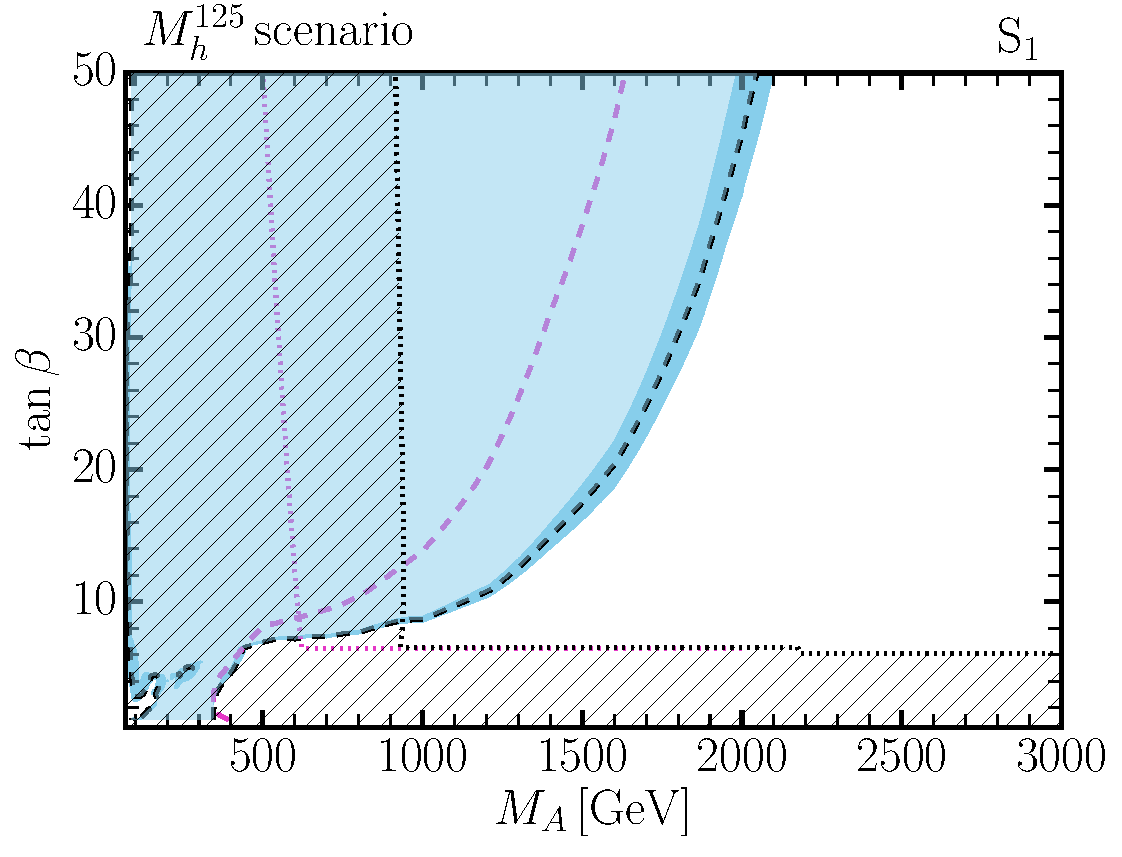
\includegraphics[width=0.5\textwidth]{section9/mh125S1_HBHS}\hfill
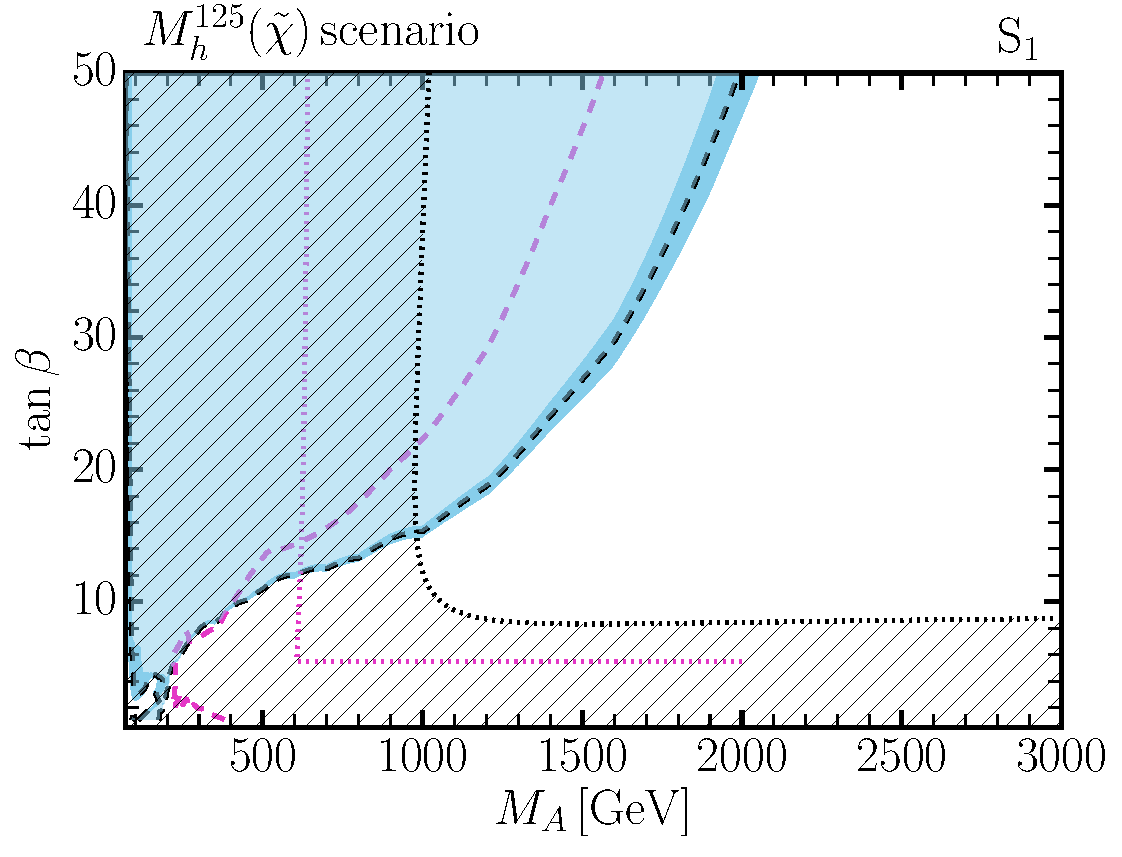
\includegraphics[width=0.5\textwidth]{section9/mh125-lc_S1_HBHS}\\
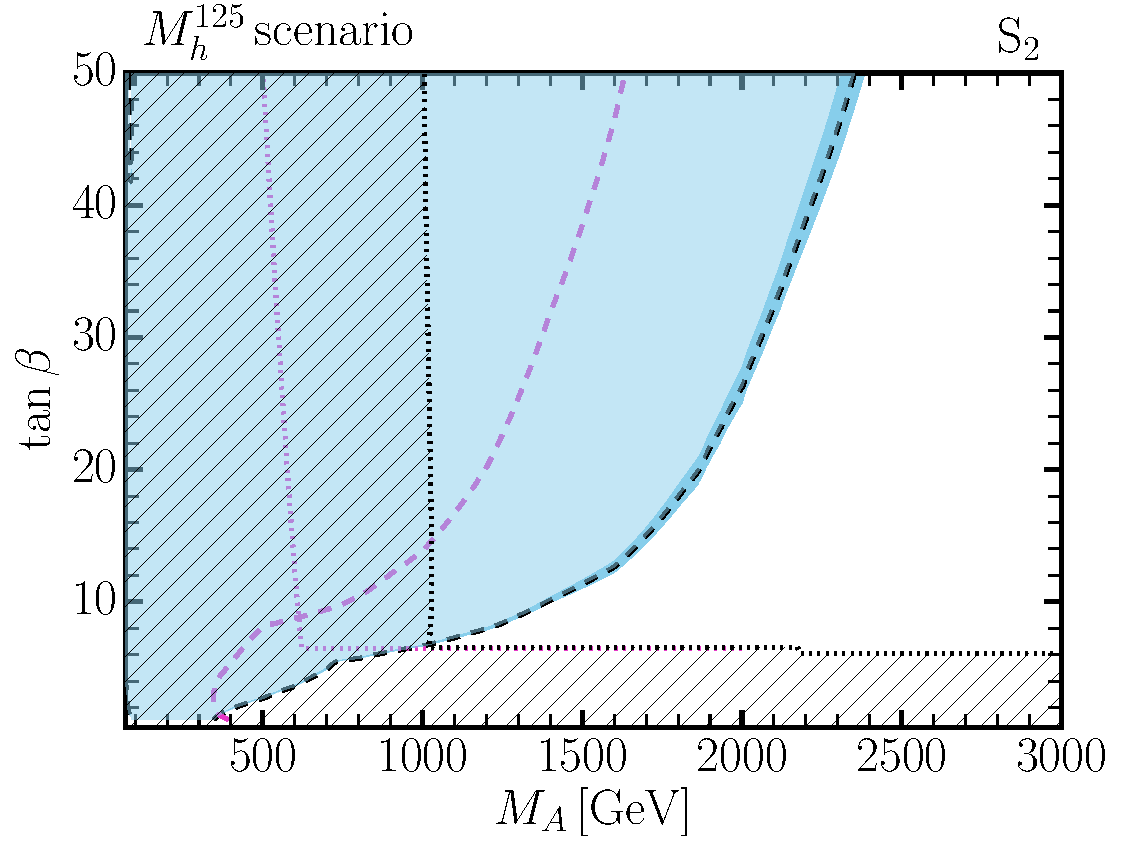
\includegraphics[width=0.5\textwidth]{section9/mh125S2_HBHS}\hfill
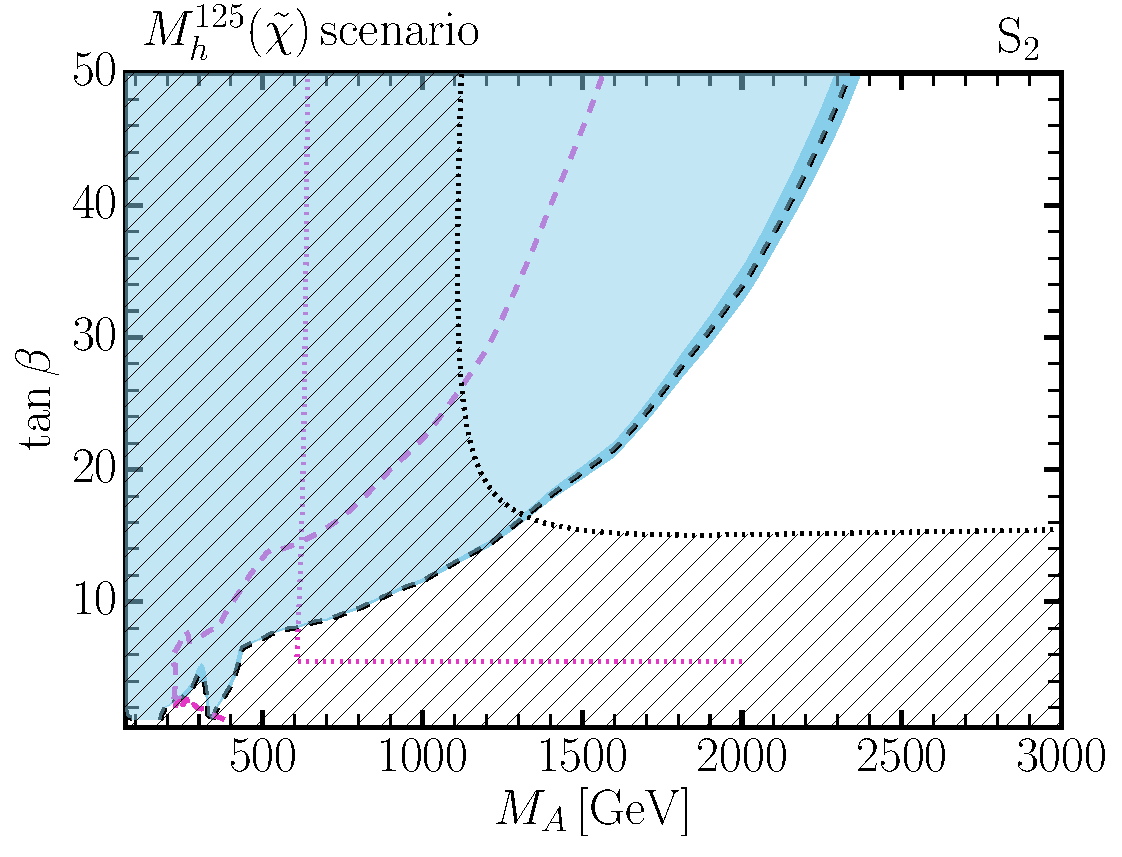
\includegraphics[width=0.5\textwidth]{section9/mh125-lc_S2_HBHS}

\end{center}
\caption{HL-LHC projections in the $M_h^{125}$ (\emph{left}) and
  $M_h^{125}(\tilde{\chi})$ (\emph{right}) scenario for the projection scenario S1 (\emph{top}) and S2 (\emph{bottom}). The dashed black curve and blue filled region indicate the HL-LHC reach via direct heavy Higgs searches in the $\tau^+\tau^-$ channel (with the dark blue region indicating the theoretical uncertainty), whereas the magenta dashed curve shows the current exclusion. The current and future HL-LHC sensitivity via  combined ATLAS and CMS Higgs rate measurements is shown as magenta and black dotted contours, respectively (the latter being accompanied with a hatching of the prospectively excluded region).}
\label{fig:bench}
\end{figure}
%%%%%%%%%%%%%%%%%%% F I G U R E %%%%%%%%%%%%%%%%%%%%%%%%%%%%%%%%%%%%%%%%%%%%%%%

Within the $M_h^{125}$ scenario the reach via measurements of the Higgs signal strengths extends to $M_A$ values of around $900~(1000)$\,GeV for S1 (S2). The horizontal contour excluding $\tan\beta$ values less than 6 is due to the light Higgs mass being below $122$\,GeV. Hence, this boundary is not changing between S1 and S2 in the $M_h^{125}$ scenario. The direct heavy Higgs searches in the $\tau^+\tau^-$ final state will probe the parameter space up to $M_A \le 2000~(2400)$\,GeV in S1 (S2) for $\tan\beta = 50$, and up to $M_A \le 1600~(1900)$\,GeV at $\tan\beta = 20$. 

The picture is somewhat different in the $M_h^{125}(\tilde{\chi})$ scenario. Here the large branching ratio of the heavy neutral Higgs boson decaying to charginos and neutralinos leads to a strongly reduced direct reach of heavy Higgs to $\tau^+\tau^-$ searches. While at large values of $\tan\beta \sim 50$  the reach is only slightly weaker than in the $M_h^{125}$ scenario, at $\tan\beta = 20$ it is significantly reduced to $M_A \le 1250~(1550)$\,GeV for S1 (S2). In order to overcome this, dedicated searches for the decays of $H$ and $A$ to charginos and neutralinos will have to be devised. On the other hand, Higgs rate measurements are an important complementary probe. In S1 they exclude
$M_A \le 1000$\,GeV and $\tan\beta \le 9$. While the bound in $M_A$
is induced through Higgs coupling modifications arising from
non-decoupling, values of $\tan\beta\le 9$ feature a too-large enhancement of the $h\to \gamma\gamma$ partial width. In the optimistic scenario S2 with reduced theoretical uncertainties these limits improve further to $M_A \ge 1100$\,GeV and $\tan\beta \gtrsim 16$, respectively.
In that case the combination of direct and indirect bounds yields
a lower limit of $M_A \ge 1300$\,GeV in the $M_h^{125}(\tilde{\chi})$ scenario.

In summary, the HL-LHC has the potential, using the combined direct and indirect reach, to probe the MSSM Higgs sector up to $M_A \sim 1000$\,GeV and possibly beyond, depending on the details of the MSSM scenario. Values larger than that, as predicted, e.g., by GUT based models~\cite{Buchmueller:2013rsa,Buchmueller:2014yva,Bechtle:2015nua,Bagnaschi:2016afc,Bagnaschi:2016xfg,Costa:2017gup} or Finite Unified Theories~\cite{Heinemeyer:2013nza,Heinemeyer:2018roq,Heinemeyer:2018zpw}, or allowed by global fits of the phenomenological MSSM~\cite{Bechtle:2016kui,Bagnaschi:2017tru} would remain uncovered. To explore these regions an energy upgrade and/or refined Higgs signal strength measurements (e.g.\ at an $e^+e^-$ collider~\cite{Moortgat-Picka:2015yla}) will be
necessary.  




\subsection{Searches for low mass Higgs bosons (below 120 GeV)}


%%%%%%%%%%%%%%%%%%%%%%%%%%%%%%%%%%
\subsubsection{Introduction}\label{sec:intro}

Many extensions of the Standard Model (SM) Higgs sector allow for new
charged and neutral Higgs bosons that can be lighter than the Higgs
boson discovered~\cite{Aad:2012tfa,Chatrchyan:2012xdj} at $\approx 125$~GeV. 
However, as the observed (heavier) Higgs boson shows itself to be 
increasingly SM-like~\cite{Falkowski:2013dza} in its couplings to $WW$
and $ZZ$ pairs~\cite{Khachatryan:2014kca,Khachatryan:2016vau,Sirunyan:2017exp,Sirunyan:2017tqd,Aaboud:2017oem,Falkowski:2013dza},
as well as to fermions~\cite{Aaboud:2018zhk,CMS:2018abb}, we are in
general pushed into an `alignment without decoupling'
limit~\cite{Gunion:2002zf,Carena:2013ooa}, which has been examined in a
number of recent
studies~\cite{Craig:2013hca,Carena:2014nza,Carena:2015moc,Bernon:2015wef,Profumo:2016zxo,Bechtle:2016kui,Haber:2017erd,Bahl:2018zmf}. In
this limit, the 125~GeV Higgs boson has SM like couplings without having
to decouple the other Higgs bosons which might be present allowing them
to be lighter than 125~GeV. In what follows we work in the alignment
without decoupling limit focusing on new Higgs bosons in the mass range
$65 - 120$~GeV, between the SM-like Higgs mass and its two body decay
threshold. 

In two Higgs doublet models (2HDM) alignment occurs when one of the
neutral CP-even Higgs mass eigenstates is approximately aligned in field
space with the direction of the vacuum expectation value
(\emph{vev})~\cite{Carena:2013ooa,Bernon:2015wef}. For non-doublet
electroweak multiplets (as well as singlets~\cite{Robens:2015gla}), one
obtains an `aligned' SM-like Higgs when the
non-doublet~\cite{Georgi:1985nv,Killick:2013mya} Higgs \emph{vev} is
small, which typically also suppresses the Higgs mixing
angle~\cite{Haber:1978jt,Hartling:2014zca}. Furthermore, in the singlet
and non-doublet multiplet cases, the new Higgs bosons are (at least
approximately) fermiophobic, making them generically harder to
detect~\cite{Akeroyd:1998ui,Akeroyd:1995hg,Delgado:2016arn,Vega:2018ddp}
either directly or indirectly as we discuss more below.  

In this review we summarize the relevant experimental constraints on
light Higgs bosons in the mass range $65 - 120$~GeV. We also discuss
models which can realize light Higgs bosons and highlight promising
search signals at the LHC. This includes searching for deviations in
Higgs couplings since, as emphasized in~\cite{Bernon:2015wef}, even in
the deep alignment regime where one might naively expect everything to
be very SM-like, precise measurements of the 125~GeV Higgs boson signal
strengths could uncover the existence of an extended Higgs sector. Some
projections for a high luminosity/high energy LHC are also made. 
The aim is to encourage new experimental analysis, targeting
specifically searches for light Higgs bosons at the HL/HE-LHC.

%%%%%%%%%%%%%%%%%%%%%%%%%%%%%%%%%%
\subsubsection{Experimental constraints on light Higgs bosons}\label{sec:limits}

In the mass range and alignment limit we consider, the most relevant
constraints for the \emph{anti}-aligned neutral Higgs bosons but with
significant couplings to SM fermions, come from CMS $b\bar{b}X$ with $X
\to \tau\bar{\tau}$ searches~\cite{Khachatryan:2015baw} as well as
ATLAS~\cite{Aad:2014vgg} and CMS~\cite{Khachatryan:2014wca} searches for
$X \to \tau\bar{\tau}$ decays in both the $gg \to X$ and $b\bar{b}X$
production modes. Similarly, the searches in the diphoton channel
  place important bounds~\cite{CMS-PAS-HIG-17-013,ATLAS-CONF-2018-025}.%
\footnote{It is interesting to note that the CMS search in the diphoton
  channel~\cite{CMS-PAS-HIG-17-013} shows an excess of events at $\sim
  96$~GeV, in the same mass range where the LEP searches in the 
  $b \bar b$ final state observed a $2\,\sigma$ excess~\cite{Schael:2006cr}.}
A recent CMS search~\cite{CMS:2015mba} for new
resonances decaying to a $Z$ boson and a light resonance, followed by 
$Z \to \ell\bar\ell$ and the light resonance decaying to $b\bar{b}$ or
$\tau\bar{\tau}$ pairs, has also been shown to impose severe
constraints~\cite{Bernon:2015wef} on light CP-even neutral Higgs
bosons. Direct searches at LEP for light neutral Higgs states produced
in pairs or in association with a $Z$ boson are also
relevant~\cite{Barate:2003sz,Abbiendi:2004gn,Schael:2006cr},
setting relevant limits on the couplings of the light Higgs to SM
gauge bosons. For
the charged Higgs bosons, LEP searches~\cite{Abbiendi:2013hk} and
$B$-physics constraints from $R_b,\,\epsilon_K,\,\Delta m_B,\,B\to
X_s\gamma$, and
$B\to\tau\nu$~\cite{Haisch:2008ar,Mahmoudi:2009zx,Gupta:2009wn,Jung:2010ik,Misiak:2015xwa}
measurements impose the most stringent constraints. These limits apply
to all 2HDMs and impose particularly severe constraints on
\emph{non}-type-I 2HDMs~\cite{Bernon:2015wef} in which there is no
fermiophobic limit.  

As emphasized in numerous studies~\cite{Ilisie:2014hea,Enberg:2016ygw,Delgado:2016arn,Degrande:2017naf,Vega:2018ddp}, the above limits are less stringent (most limits can be rescaled) when the Higgs bosons have highly suppressed couplings to SM fermions as can happen in the type-I 2HDM~\cite{Haber:1978jt} in the large $\tan\beta$ limit~\cite{Akeroyd:1995hg}. For non-doublet extended Higgs sectors one automatically has suppressed couplings to SM fermions when the non-doublet \emph{vev} is small (or mixing angle in the case of singlets) since they only enter (if at all) through mixing with the SM-like Higgs boson~\cite{Killick:2013mya}.~In the case of fermiophobia, the most robust probes of neutral Higgs bosons are inclusive diphoton~\cite{Delgado:2016arn,Degrande:2017naf,Vega:2018ddp} and multiphoton searches~\cite{Akeroyd:2005pr,Abdallah:2003xf,Aaltonen:2016fnw} which utilize the Drell-Yan pair production channel of a charged and neutral Higgs boson.~Constraints from electroweak (EW) precision data~\cite{Baak:2011ze,ALEPH:2010aa} also apply with the primary effect being that the neutral and charged Higgs bosons are constrained to be not too different in mass.  

%%%%%%%%%%%%%%%%%%%%%%%%%%%%%%%%%%
\subsubsection{Models with light Higgs bosons}\label{sec:models}

A number of recent studies of the alignment without decoupling limit in
2HDMs have been performed which consider the case where the SM-like
Higgs boson is not the lightest scalar. As shown
in~\cite{Ilisie:2014hea,Bernon:2015wef,Enberg:2016ygw,Arhrib:2017wmo,Arbey:2017gmh,Bhatia:2017ttp,Fox:2017uwr,Haber:2017erd,Haisch:2017gql},
for type-I 2HDMs there are regions of parameter space where, along with
the light CP-even scalar, both the charged and neutral CP-odd Higgs
bosons can be below the SM-like Higgs mass while satisfying the
constraints discussed above. This is in contrast to type-II 2HDM,
where combined constraints from $B$ meson
decays~\cite{Misiak:2015xwa} and EW precision
constraints~\cite{Peskin:1991sw} require the charged and CP-odd neutral
Higgs bosons to be much heavier than the mass range we consider here. Within the MSSM however, the additional particle content results in
  substantially weaker limits from $B$~meson decays and EW data.
In general the allowed regions of parameter space in the type-I 2HDM is
much larger than in other 2HDMs~\cite{Bernon:2015wef,Haber:2017erd},
again due to the presence of a fermiophobic limit at large $\tan\beta$
which opens up more regions of parameter space. 

In the MSSM which is a type-II 2HDM, the alignment without decoupling
limit~\cite{Carena:2013ooa} requires accidental cancellations between
tree level and radiative corrections in the Higgs mass
matrix~\cite{Bechtle:2016kui,Haber:2017erd}. It was shown that a tuning of $\sim 10\%$ is sufficient to find agreement with the Higgs-boson rate measurements~\cite{Bechtle:2016kui}. Depending on the level of alignment required, this can lead to a highly constrained parameter space, especially in the case where the SM-like Higgs is the heavier of the CP-even neutral scalars. In particular, after accounting for all relevant experimental constraints (as well as theoretical uncertainties) recent studies~\cite{Bahl:2018zmf} of the alignment without decoupling limit of the MSSM~\cite{Carena:2013ooa} defined a benchmark plane of allowed parameter space with $\tan\beta \sim 5 - 6$ (and very large values of $\mu$) in which the light CP-even Higgs can be between  $\sim 60 - 100$~GeV if the charged Higgs mass is between $\sim 170 - 185$~GeV and the neutral CP-odd Higgs is $\sim 130 - 140$~GeV. Still larger allowed regions are expected in a global scan, as performed in~\cite{Bechtle:2016kui}.
Recent studies of the NMSSM~\cite{Carena:2015moc,Domingo:2018uim} and
$\mu\nu$SSM~\cite{Biekotter:2017xmf} have also examined the alignment
without decoupling limit finding a larger allowed parameter space than in the
MSSM due to an additional gauge singlet Higgs (or right handed scalar
neutrino). 

For models with non-doublet multiplets the most well known are those involving electroweak triplets. In particular, Higgs triplet models with custodial symmetry~\cite{Sikivie:1980hm}, as in the famous Georgi-Machacek (GM) model~\cite{Georgi:1985nv,Chanowitz:1985ug,Gunion:1989ci,Gunion:1990dt,Hartling:2014zca} or its supersymmetric incarnations~\cite{Cort:2013foa,Garcia-Pepin:2014yfa,Vega:2017gkk}, have been well studied due to their ability to easily satisfy constraints from electroweak precision data. Recent studies~\cite{Davoudiasl:2004aj,Vega:2017gkk,Vega:2018ddp} have shown that GM-like models can allow for light neutral and charged scalars below the SM-like Higgs boson mass. In the alignment limit implied by Higgs coupling measurements, the triplet Higgs \emph{vev} is constrained to be small though it can still much larger than non-custodial cases~\cite{Tanabashi:2018oca,Haber:1999zh} which are constrained by measurements of the $\rho$ parameter. Custodial symmetry also ensures that the neutral and charged components of the Higgs multiplet have (at least approximately) degenerate masses, making them more difficult to detect due to soft decay products~\cite{Buckley:2009kv,Ismail:2016zby}. For these anti-aligned and fermiophobic Higgs bosons, recent studies have emphasized di- and multi-photon searches~\cite{Aaltonen:2016fnw,Delgado:2016arn,Brooijmans:2016vro,Vega:2018ddp} as robust probes of this scenario.

%%%%%%%%%%%%%%%%%%%%%%%%%
\subsubsection{Phenomenology of light anti-aligned Higgs bosons}\label{sec:pheno}

In the alignment limit, single electroweak production mechanisms for the
additional `anti-aligned' neutral Higgs bosons (or small \emph{vev} and Higgs mixing for non-doublets), such as vector boson fusion (VBF) or associated vector boson production, necessarily become suppressed. Thus the dominant production mechanisms become gluon fusion or associated $b\bar{b}$ production when there is a significant coupling to SM quarks. However, these production mechanisms become suppressed when the couplings to fermions are negligible\,\footnote{Of course if they couple to some not too heavy colored BSM particles, gluon fusion could open back up.}, as can happen in type-I 2HDM in the large $\tan\beta$ limit~\cite{Akeroyd:2003bt} or non-doublet electroweak sectors which are generically fermiophobic. The same is true for the light charged Higgs bosons production channels $t \to H^\pm b$ and $pp \to H^\pm t b$ which are also obsolete in the fermiophobic limit. Note that for charged scalars coming from larger than doublet representations we can also have $W^\pm Z \to H^\pm$ VBF production, but this is again suppressed in the small non-doublet \emph{vev} and Higgs mixing limit. 


%%%%%%%%%%%%%%%%%%%%%%%%%
\subsubsubsection{Pair Production as a discovery channel}\label{sec:pair}

A different option that offers new experimental opportunities is
  the Drell-Yan Higgs pair production mechanism. Any extension of the SM Higgs sector by electroweak charged scalars will possess the pair production channels mediated by $W$ and $Z$ bosons and which are not present in the SM. Furthermore, as emphasized in~\cite{Akeroyd:2003bt,Akeroyd:2003xi,Akeroyd:2003jp,Ilisie:2014hea,Delgado:2016arn,Vega:2018ddp}, even in the alignment and fermiophobic limits, this production mechanism is not suppressed and can be as large as $\sim 10\,pb$ at 13~TeV and $\sim 50\,pb$ and 27~TeV in the mass range we consider (see~\ref{HHprod}). Thus, Drell-Yan Higgs pair production can be as large or even dominate over single  production mechanisms, for both charged and neutral Higgs bosons. Despite this, the Drell-Yan Higgs pair production mechanism has been largely overlooked in experimental searches with the lone exception being a recent CDF analysis of Tevatron four photon data~\cite{Aaltonen:2016fnw} searching for fermiophobic Higgs bosons.  

The Drell-Yan pair production mechanism is mediated by the vector-Higgs-Higgs coupling. In the alignment limit, this will have vertices that are maximized in this limit and depend only on electroweak couplings and quantum numbers, while some vertices will go to zero depending on which Higgs pairs are being produced~\cite{Akeroyd:2003bt,Akeroyd:2003xi,Akeroyd:2003jp,Ilisie:2014hea,Delgado:2016arn,Vega:2018ddp}. Thus for the non-zero cases the vertex can be written schematically as,
%
\bea\label{eqn:gvhh}
g_{WH_M^\pm H_N^0} \equiv i g 
\, C_N (p_1 - p_2)^\mu ,~~
g_{ZH_M^0H_N^0} \equiv i \frac{g}{c_W} 
\, C_N (p_1 - p_2)^\mu ,
\eea
%
where $C_N$ is fixed by the $SU(2)_L\times U(1)_Y$
representation~\cite{Georgi:1985nv,Akeroyd:2003bt,Akeroyd:2010eg,Cort:2013foa,Hartling:2014zca} and $p_{1}, p_{2}$ are the four momenta of the incoming and outgoing scalar momenta. Here $H_N^0$ stands for any neutral Higgs boson and can include CP-even or CP-odd and similarly for $H_M^\pm$ in the case of charged Higgs bosons. There is also a photon mediated channel when both Higgs bosons are charged, but we focus on cases where at least one is neutral. In~\ref{HHprod} we show the leading order $q\bar{q} \to V \to H_M^{\pm,0} H_N^0$ (including \emph{pdfs}) cross section $\times\, C_N^{-2}$ for the $W$ mediated (blue solid) and $Z$ mediated (black dashed) channels at the LHC with $\sqrt{s}=13$~TeV (left) and $\sqrt{s}=27$~TeV (right) in the mass range $60 - 125$~GeV. They are computed with Madgraph~\cite{Alwall:2014hca} using a modified version of the GM model implementation of~\cite{Hartling:2014xma} and rescaling appropriately. There are also NLO contributions which may generate $\gtrsim \mathcal O(1)$ K-factors for Higgs pair production~\cite{Eichten:1984eu,Dawson:1998py,Degrande:2015xnm}, but are not included. We show four cases for mass splittings  of $\Delta M \equiv M_{H^{\pm,0}_M} - M_{H_N^0} = 0, 100, 200, 300$~GeV as labeled in plot.  
%%%%%
\begin{figure}[tbh]
\begin{center}
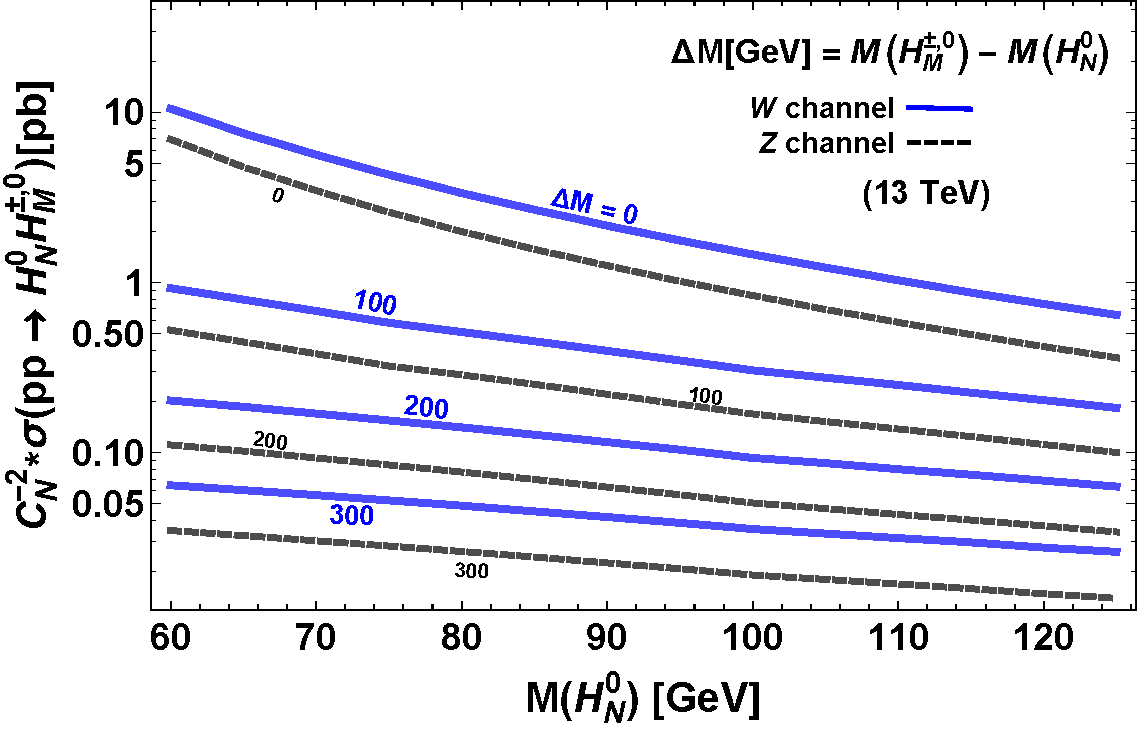
\includegraphics[scale=.403]{FigsLowMassHiggs/CxnVsMHoDelM_13TeV.pdf}
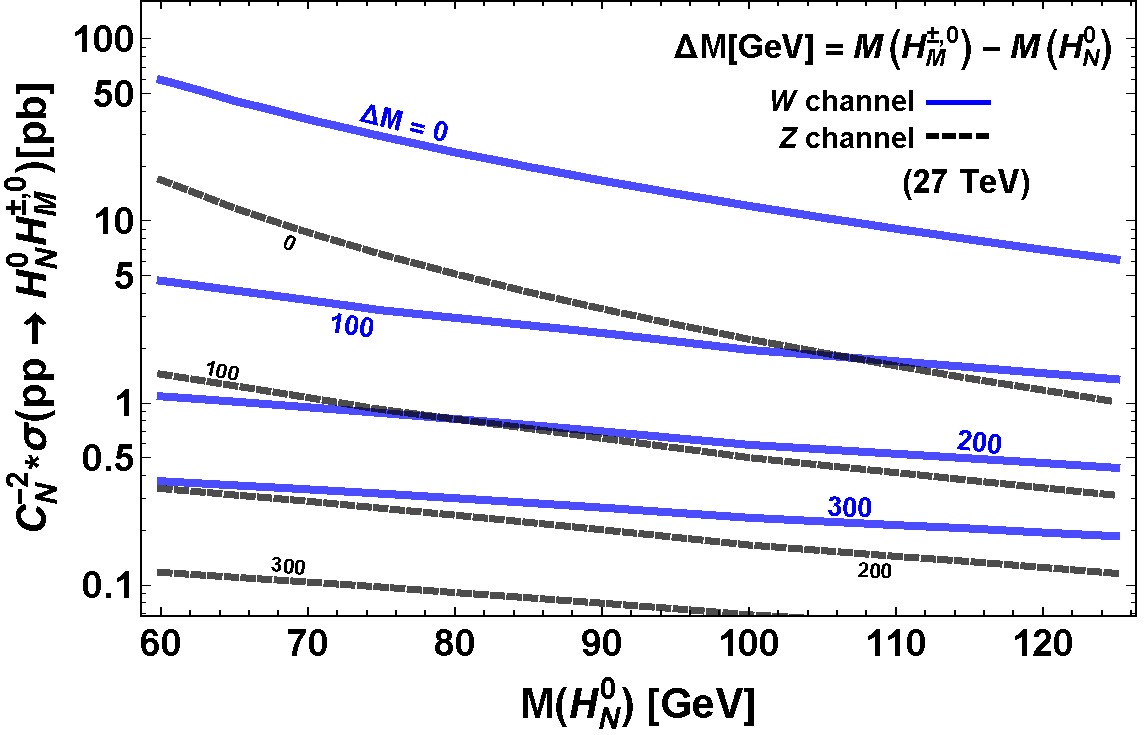
\includegraphics[scale=.4]{FigsLowMassHiggs/CxnVsMHoDelM_27TeV.pdf}
\end{center}
\caption{Leading order cross sections (with \emph{pdfs}) for the $q\bar{q} \to V \to H_M^{\pm,0} H_N^0$ Higgs pair production mechanism mediated by $W$ (blue solid) and $Z$ (black dashed) bosons at the LHC for $\sqrt{s}=13$~TeV (left) and $\sqrt{s}=27$~TeV (right) in the mass range $60 - 125$~GeV. We show three cases for mass splittings $\Delta M \equiv M_{H^{\pm,0}_M} - M_{H_N^0}= 0, 100, 200, 300$~GeV as labeled in plot and have factored out an overall group theory factor $C_N$ (see~\ref{gvhh}). The curves for a particular model can be obtained by rescaling with $(C_N)^2$ which is fixed by the $SU(2)_L\times U(1)_Y$ representation.} 
\label{fig:HHprod}
\end{figure}
%%%%%

The dominant decay modes of the neutral Higgs bosons will be to $b\bar{b}$ and $\tau\bar{\tau}$ when there is a significant coupling to SM fermions. In the fermiophobic case, the Higgs bosons can have large branching ratios into EW gauge bosons and in particular photons at low masses. The less emphasized $Z\gamma$ channel may also offer promising opportunities~\cite{Degrande:2017naf}. Inclusive searches for resonances can then be combined with the Drell-Yan production channel to put relatively robust bounds on branching ratios in extended Higgs sectors as done in~\cite{Delgado:2016arn,Vega:2018ddp} for the case of decays into diphotons. For the charged Higgs bosons combing Drell-Yan pair production with decays into $W\gamma$~\cite{Ilisie:2014hea,Degrande:2017naf} or four photon signals~\cite{Aaltonen:2016fnw} offer promising search channels.


%%%%%%%%%%%%%%%
\subsubsubsection{Suggestions for searches at the HL/HE-LHC}

We briefly summarize search strategies for (anti)-aligned light
Higgs bosons at the (HL/HE) LHC. This is in addition to continuing
and updating current searches in the mass range we consider, including
$\tau\tau,\,\gamma\gamma,\,b\bar{b}$ searches based on gluon fusion and
$\tau\tau$ searches based on associated $b\bar{b}$
production~\cite{Aad:2014vgg,Khachatryan:2014wca,Khachatryan:2015baw} as
well as recent CMS searches~\cite{CMS:2015mba} for $A \to Zh$ with $Z
\to \ell\bar\ell$ and $h\to \tau\tau, bb$.  

%%%%%%%%%%%%%%%%
%\subsection{Suggestions for searches at the HL/HE-LHC}

\begin{itemize}
\item Push current conventional Higgs searches in $WW$ and $ZZ$, which
  currently~\cite{Khachatryan:2015cwa,Sirunyan:2018qlb} do not go below
  $\sim 130$~GeV, to as low a mass as possible, ideally down to $\sim
  65$~GeV. As emphasized in~\cite{Delgado:2016arn,Vega:2018ddp}, this
  can help to rule out cases of a fermiophobic Higgs boson with
  suppressed couplings to photons, which could otherwise escape
  detection. Similarly, heavier Higgs bosons with the ``remaining''
  coupling to SM gauge bosons could be detected.

\item Combine \emph{inclusive} searches for resonances with the
  `universal' Drell-Yan Higgs pair production channel to put robust
  bounds on allowed branching ratios to $\tau\tau$, $b\bar{b}$, $Z\gamma$ and
  $\gamma\gamma$ final states. In the alignment limit,
  these bounds depend only on electroweak couplings and can be applied
  to any extended Higgs boson sector (with appropriate rescaling), in
  some cases providing the strongest limits~\cite{Delgado:2016arn,Vega:2018ddp}.

\item Utilizing the Drell-Yan Higgs pair production mechanism, dedicated
  LHC searches for more optimized, but model dependent signals such as
  $4\gamma + V^\ast$~\cite{Akeroyd:2003bt,Aaltonen:2016fnw,Arhrib:2017wmo},
  $4\gamma + V^\ast V^\ast$~\cite{Akeroyd:2003bt}, $3\gamma +
  V^\ast$ where in the last case dedicated phenomenological studies are
  lacking. 

\item Search for $\tau\tau$, $b\bar{b}$, or $\gamma\gamma$ plus missing
  energy as well as mono photon or mono lepton plus missing energy final
  states to cover cases where neutral Higgs may have an invisible
  decay. In particular the $\gamma\gamma$ channel appears to be
  very promising (especially in view of a potential signal at 
  $\sim 96$~GeV~\cite{CMS-PAS-HIG-17-013}).
 
\end{itemize}




\subsection{Sensitivity to heavy Higgs bosons from the 2HDM}

\begin{center}
 {K. Mimasu$^{1}$, Jose Miguel No$^{2}$ \\
}
%\noindent
 {\small $^{1}$Universite catholique de Louvain, Chemin du Cyclotron, 2, B-1348 Louvain-la-Neuve, Belgium \\
 $^{2}$Instituto de Fisica Teorica, IFT-UAM/CSIC, Cantoblanco, 28049, Madrid, Spain}
\end{center}

\subsubsection{Introduction}

Searches for heavy scalars are highly complementarity to coupling measurements of the 125 GeV Higgs $h$ as probes of extended Higgs sectors. For 2HDM scenarios, di-boson search channels $H \to WW$, $ZZ$, $hh$ probe the parameter space for which the 125 GeV Higgs is not SM-like, in combination with Higgs coupling measurements.
However for a SM-like 125 GeV Higgs, corresponding to the alignment limit of 2HDMs~\cite{Gunion:2002zf}, these channels suffer a significant loss in  
sensitivity since the couplings $HVV$ ($V = W^{\pm},\,Z$) and $Hhh$ vanish in such a limit. In this case, searches for heavy scalars through non-standard decay channels~\cite{Coleppa:2014hxa,Dorsch:2014qja,Li:2015lra,Kling:2016opi} 
as well as through fermionic decay channels~\cite{Craig:2015jba,Gori:2016zto} become the primary avenue to find these new states, and are crucial to cover the parameter space of aligned 2HDMs.

For Higgs sectors with several new states beyond the SM, as in the 2HDM, 
non-standard ``Higgs-to-Higgs" decays occur between these BSM scalars for sizable splittings among them, yielding the leading probe of aligned 
2HDM scenarios in this case~\cite{Dorsch:2016tab}. 
Focusing here in the 2HDM neutral scalars $A/H$, such signatures include 
$A/H\to Z H/A$ ($Z \to \ell \ell$, $H/A \to \bar{b}b, \tau\tau$)~\cite{Coleppa:2014hxa,Dorsch:2014qja} and 
$H \to A A \to b\bar{b} b\bar{b}, b\bar{b} \tau\tau$~\cite{Brooijmans:2018xbu}.
There exists a very strong interplay between these and searches for $H/A$ in fermionic decay channels, mainly  
$H/A \to \tau\tau$, depending on the mass splitting among the new scalars.

\subsubsection{2HDM Summary}

Relevant aspects of the 2HDM (overlap with Carlos and Nausheen's contribution) Consider a general 2HDM scalar potential 
with a softly broken $\mathbb{Z}_2$ symmetry (and no CP violation)  
%
\begin{eqnarray}	
\label{2HDM_potential}
V(H_1,H_2) &= &\mu^2_1 \left|H_1\right|^2 + \mu^2_2\left|H_2\right|^2 - \mu^2\left[H_1^{\dagger}H_2+\mathrm{h.c.}\right] 
+\frac{\lambda_1}{2}\left|H_1\right|^4 +\frac{\lambda_2}{2}\left|H_2\right|^4 \nonumber \\
&+& \lambda_3 \left|H_1\right|^2\left|H_2\right|^2
+\lambda_4 \left|H_1^{\dagger}H_2\right|^2+ \frac{\lambda_5}{2}\left[\left(H_1^{\dagger}H_2\right)^2+\mathrm{h.c.}\right]\, . 
\end{eqnarray}
%
Physical scalar sector of a 2HDM comprised of $h$ (which we assume here to be the 125 GeV Higgs), $H$, $A$ and $H^{\pm}$. 
Types of 2HDM, regarding the couplings of the two doublets $H_{1,2}$ to fermions: By convention, up-type quarks couple to $H_{2}$. In Type I 2HDM all the other fermions also couple to $H_{2}$, while for Type II down-type quarks and leptons couple\footnote{Two more possibilities (depending on coupling of leptons w.r.t.~down-type quarks), but we focus here on Types I and II.} to $H_{1}$.
Parameters $t_{\beta} \equiv \mathrm{tan}\,\beta$ and $c_{\beta -\alpha} \equiv \mathrm{cos}\,(\beta-\alpha)$ control strength of the couplings 
of $h$, $H$, $A$ to gauge bosons and fermions. We denote the couplings normalized to the SM values (of $h_{\mathrm{SM}}$) by $\kappa$-factors ($\kappa_V$ for gauge bosons, $\kappa_u$ for up-type quarks, $\kappa_d$ for 
down-type quarks, $\kappa_{\ell}$ for charged leptons), which read 
%
 \begin{equation}
 \label{t:kappas}
 \mathrm{Type}\,\mathrm{I}:\,\left\lbrace
 \begin{array}{l}
 \kappa^h_V = s_{\beta-\alpha} \\
 \kappa^h_u = \kappa^h_d = \kappa^h_{\ell} = t^{-1}_{\beta}c_{\beta-\alpha} + s_{\beta-\alpha}  \\
 \kappa^{H}_V = - c_{\beta-\alpha} \\
 \kappa^{H}_u = \kappa^{H}_d = \kappa^{H}_{\ell} = t^{-1}_{\beta}s_{\beta-\alpha} - c_{\beta-\alpha}  \\
 \kappa^{A}_u = - \kappa^{A}_d = - \kappa^{A}_{\ell} = t^{-1}_{\beta}
 \end{array}
 \right.
 \quad
  \mathrm{Type}\,\mathrm{II}:\,\left\lbrace
 \begin{array}{l}
 \kappa^h_V = s_{\beta-\alpha} \\
 \kappa^h_u = t^{-1}_{\beta}c_{\beta-\alpha} + s_{\beta-\alpha}  \\
 \kappa^h_d = \kappa^h_{\ell} = s_{\beta-\alpha} - t_{\beta}\,c_{\beta-\alpha}\\
 \kappa^{H}_V = - c_{\beta-\alpha} \\
 \kappa^{H}_u = t^{-1}_{\beta}s_{\beta-\alpha} - c_{\beta-\alpha}  \\
 \kappa^{H}_d = \kappa^{H}_{\ell} = -t_{\beta}\,s_{\beta-\alpha} - c_{\beta-\alpha}  \\
 \kappa^{A}_u = t^{-1}_{\beta}\\
 \kappa^{A}_d = \kappa^{A}_{\ell} = t_{\beta}
 \end{array}
 \right.
\end{equation}
%
For $c_{\beta -\alpha} \to 0$ (alignment limit~\cite{Gunion:2002zf}) 
$h$ has SM-like couplings to gauge bosons and fermions ($\kappa^h_i \to 1$, yielding $h \to h_{\mathrm{SM}}$), while the coupling of $H$ to gauge bosons $V = W^{\pm},Z$ vanishes ($\kappa^{H}_V \to 0$).

\subsubsection{$m_A > m_H$: searches for $A \to Z H$}

Here we obtain the present limits on the 2HDM in the alignment limit from the $\sqrt{s} = 13$ TeV ATLAS $A \to Z H$ search~\cite{Aaboud:2018eoy} with $36.1$ fb$^{-1}$ (there are also CMS searches at 8 TeV with $19.8$ fb$^{-1}$~\cite{Khachatryan:2016are} and at 13 TeV with $2.3$ fb$^{-1}$~\cite{CMS:2016qxc}) in the $\ell \ell b \bar{b}$ final state, and present sensitivity projections of this search for HL-LHC and HE-LHC. The present limits and future projections are derived in the ($m_A$, $m_H$, $\mathrm{tan}\beta$) parameter space. 

For the HL-LHC, we first perform a sensitivity projection to $\sqrt{s} = 13$ TeV with $\mathcal{L} = 3000$ fb$^{-1}$, for $m_A = m_H + 100$ GeV, $m_A = m_H + 200$ GeV, $m_A = m_H + 300$ GeV as benchmarks. 
In figure~\ref{AZH_HL-LHC} (left) our sensitivity projection is obtained through a $\sqrt{\mathcal{L}}$ rescaling of the present ATLAS expected 
sensititivy, assuming that the background uncertainties are statistically dominated. In figure~\ref{AZH_HL-LHC} (right) we instead assume a $x\%$ of background systematics (coming dominantly from $Z +$ jets) in our projections, and use xxx as signal significance.

Mind the region where $\Gamma_A/m_A > 20\%$!

\begin{figure}[h]
\begin{center}
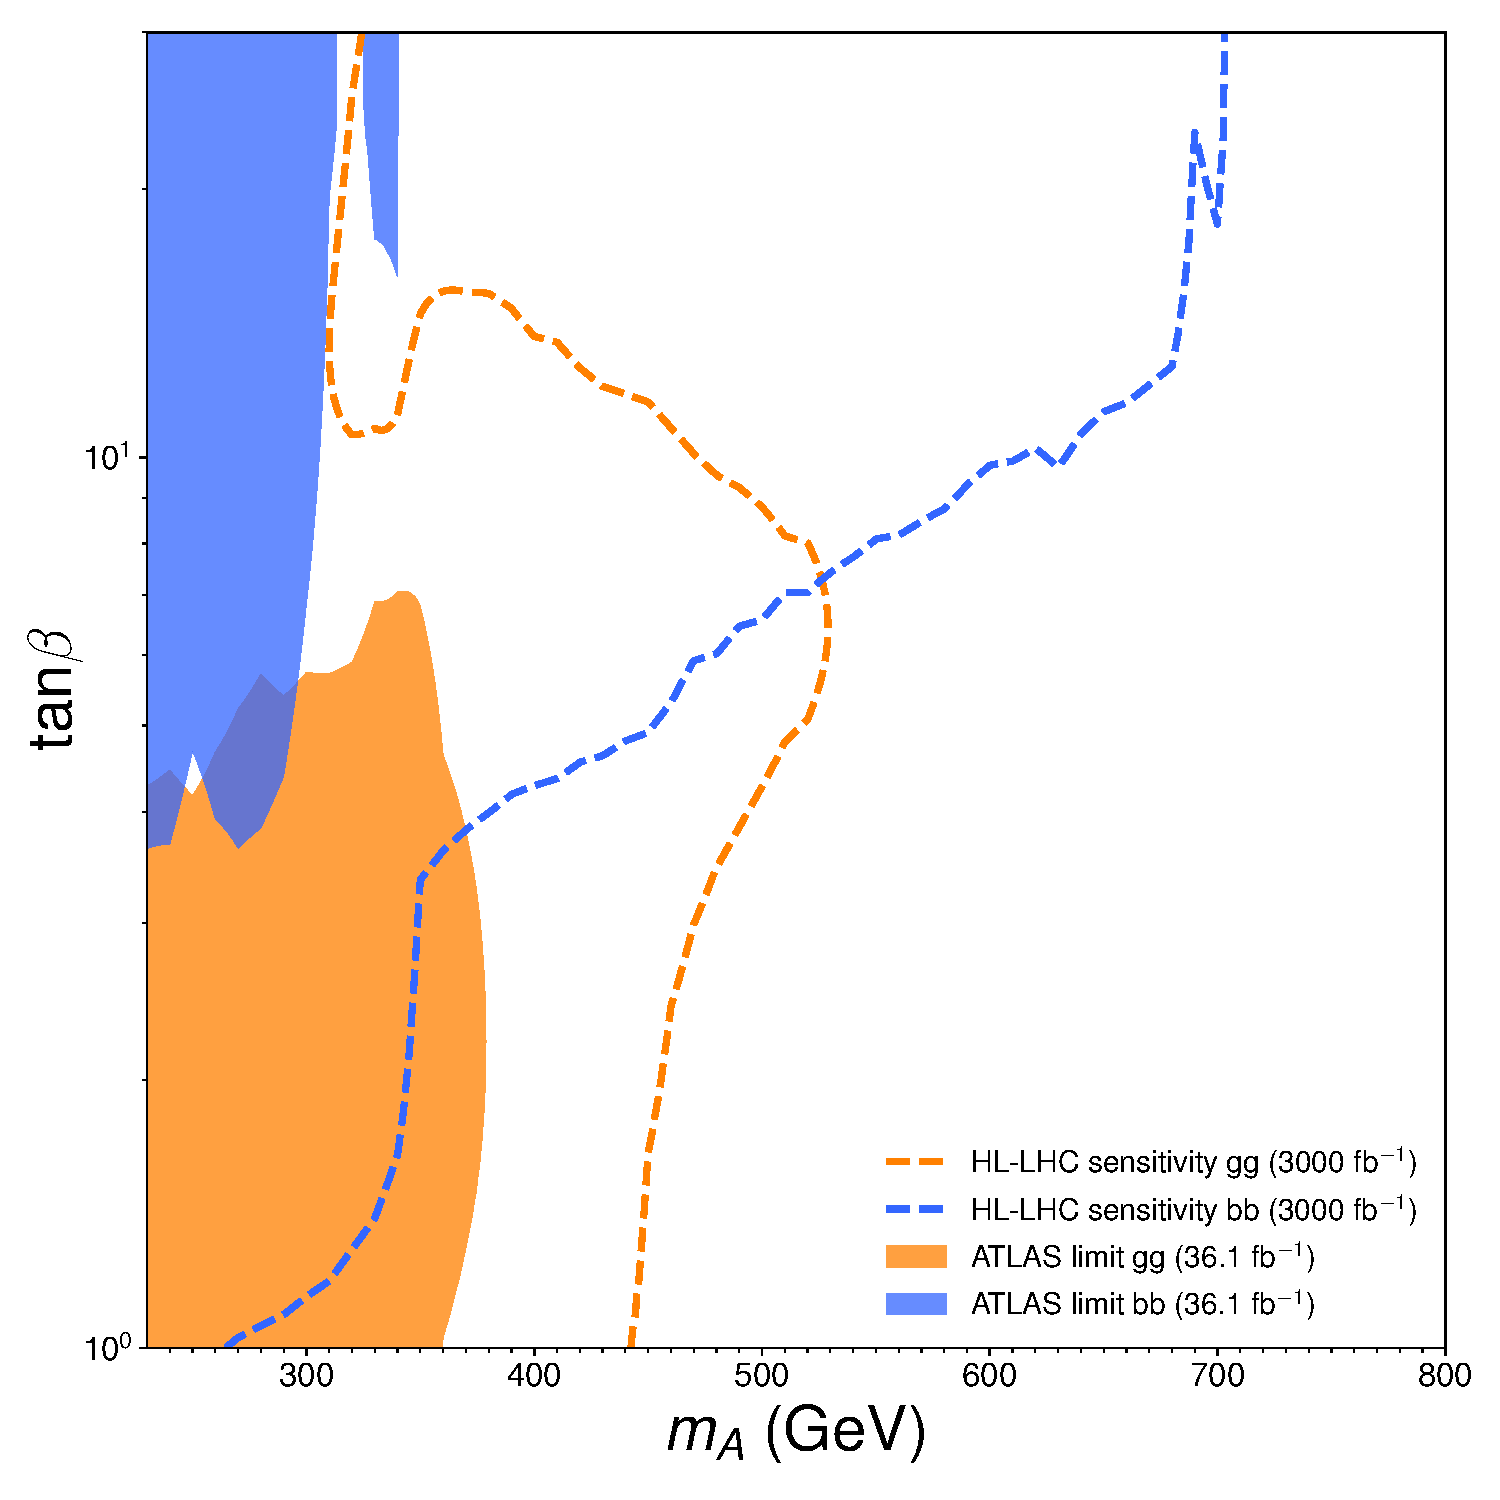
\includegraphics[width=0.48\textwidth]{\main/section9/2HDM_AZH_Plot_Statistics.pdf}
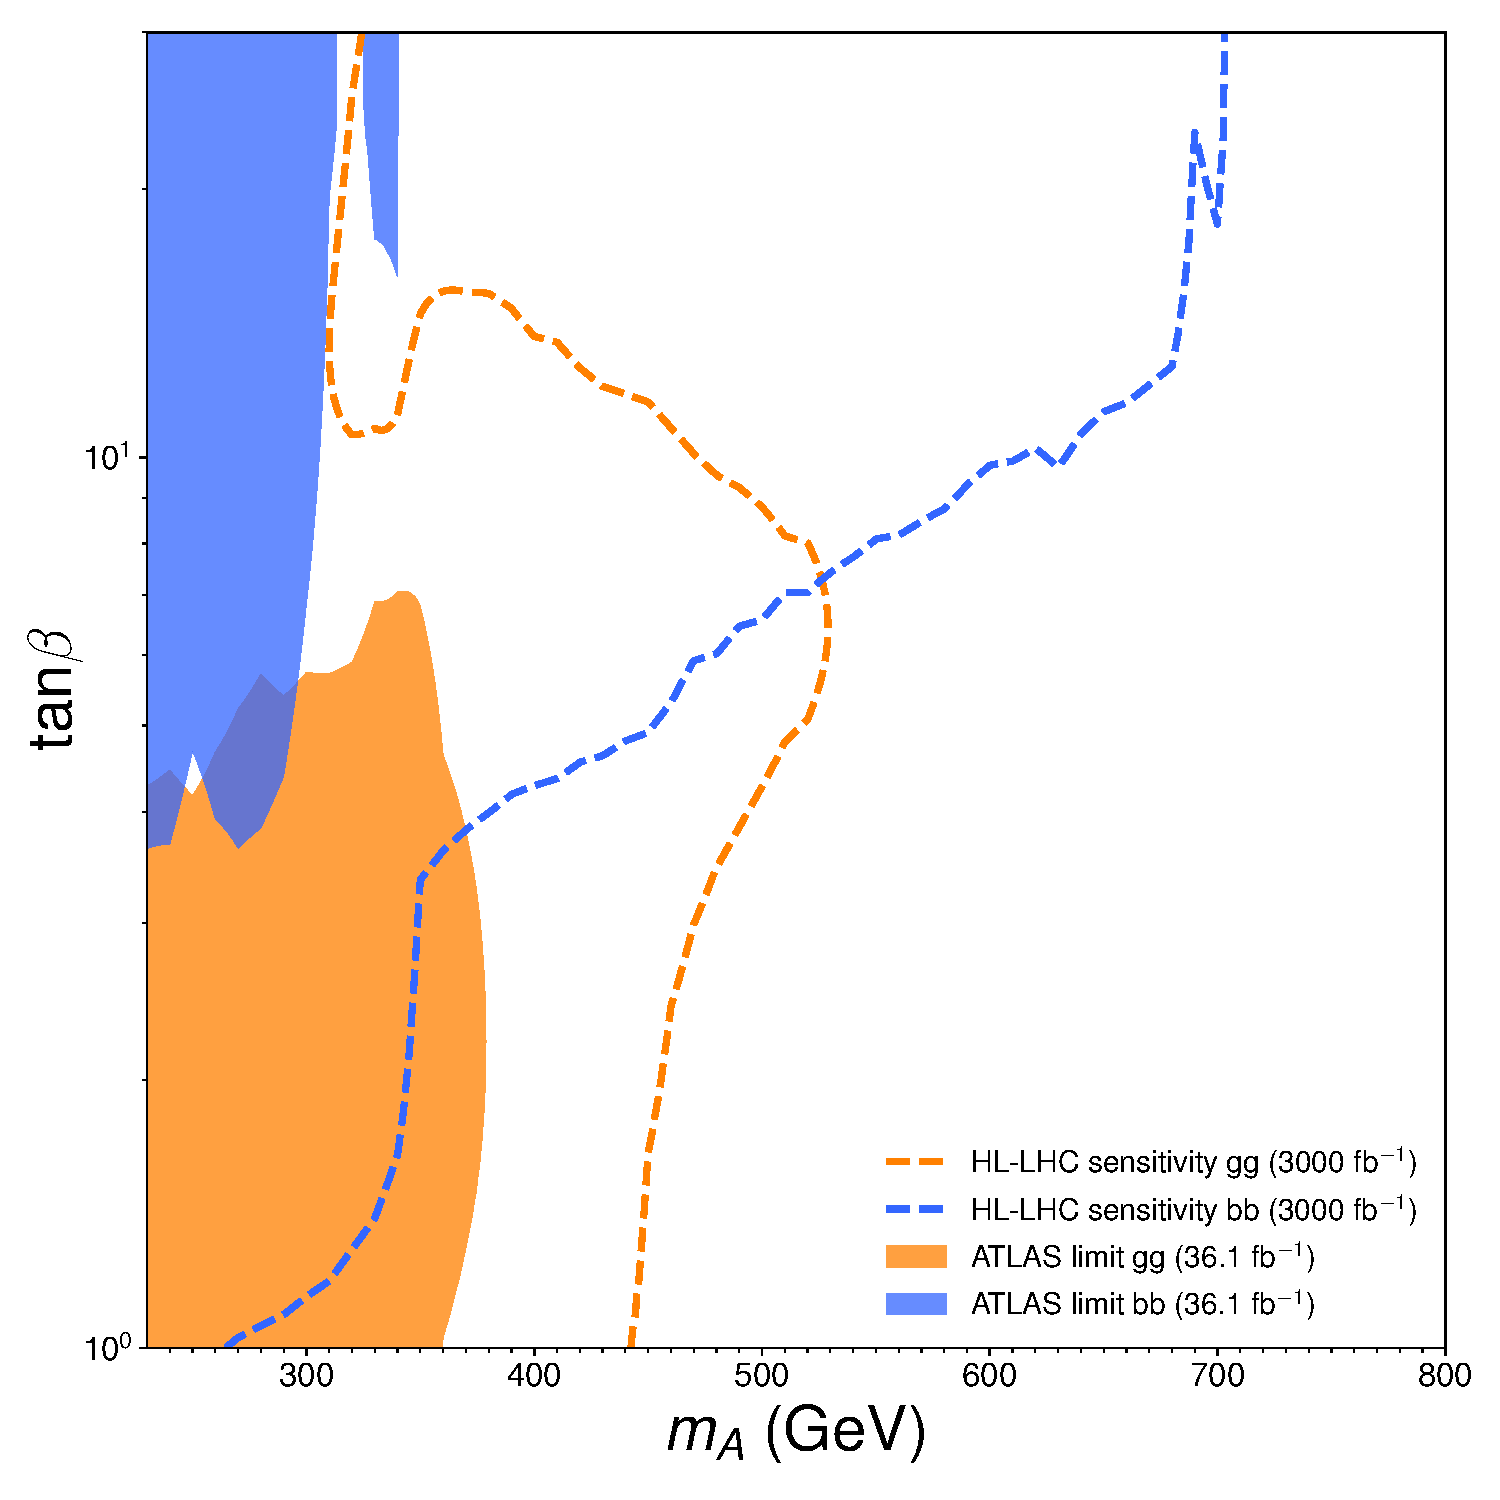
\includegraphics[width=0.48\textwidth]{\main/section9/2HDM_AZH_Plot_Statistics.pdf}
\caption{\small Left: Present (solid) and projected (dashed)  $95\%$ C.L. exclusion sensitivity for $p p \to A \to Z H \to \ell\ell b \bar{b}$ in the 
in the ($m_{A}$, tan$\beta$) plane for $m_A = m_H +100$ GeV, from 
gluon fusion (orange) and $bb$-associated production (blue). Right: \textcolor{red}{(Placeholder for the limits with systematics)}.}
\label{AZH_HL-LHC}
\end{center}
\end{figure}


\subsubsection{$m_H > m_A$: searches for $H \to Z A$ and $H \to A A$}

The analysis above can be also applied to $H \to Z A$, bearing in mind the po
ssibility of the competing decay $H \to A A$. For $H \to A A$ there are no present ATLAS/CMS experimental studies\footnote{We however note there are existing LHC analyses for $h \to A A$, with $h$ the 125 GeV Higgs boson (see e.g.~\cite{Khachatryan:2017mnf}).} but there is an existing sensitivity study~\cite{Brooijmans:2018xbu} based on the 13 TeV 
resonant di-Higgs CMS analysis~\cite{CMS:2017xxp} (see also~\cite{CMS:2016tlj}).

Following~\cite{Brooijmans:2018xbu}, we particularize the search $H\to A A \to 4 b$ for $m_{A} \in [65,\, 290]$~GeV (for which the multijet background is provided by CMS) and $m_{H} \in [m^{\mathrm{min}}, m^{\mathrm{max}}] = [3.2\times m_{A}, 9.6\times m_{A}]$ (MMR selection of~\cite{CMS:2017xxp}, validated in~\cite{Brooijmans:2018xbu}). The $95\%$ C.L. cross section times branching ratio exclusion sensitivity (in fb) for $p p \to H \to A A \to b \bar{b} b \bar{b}$ in the ($m_{H}$, $m_{A}$) plane, for LHC 13 TeV with an integrated luminosity of 35.9 fb$^{-1}$ is given in 
Figure~\ref{Fig_HAA_2D_Limits}. We Convert this into the 2HDM parameter space in Figure... 


Regarding extrapolation to HL-LHC and HE-LHC...

Mind the region where $\Gamma_H/m_H > 20\%$!

\begin{figure}[h]
\begin{center}
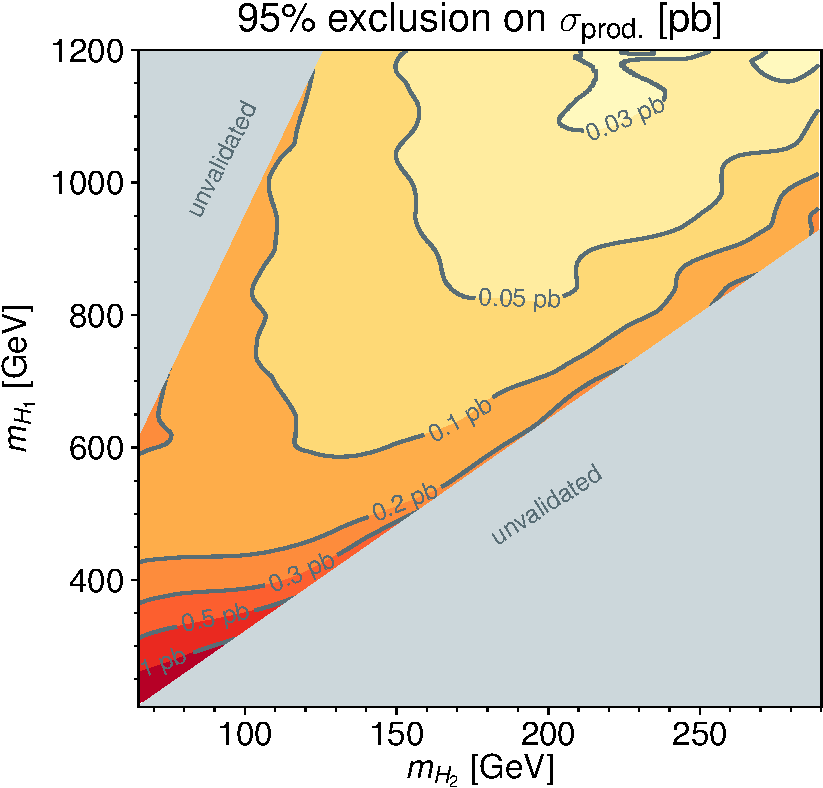
\includegraphics[width=0.65\textwidth]{\main/section9/95_exclusion_map_HAA.pdf}
\caption{\small Estimated $95\%$ C.L. $\sigma \times$ BR exclusion sensitivity for $p p \to H \to A A \to b \bar{b} b \bar{b}$ 
in the ($m_{H_1} = m_H$, $m_{H_2} = m_A$) plane for LHC 13 TeV with an integrated luminosity of 35.9 fb$^{-1}$ \textcolor{red}{(Placeholder for the 
2HDM interpretation of these limits)}.}
\label{Fig_HAA_2D_Limits}
\end{center}
\end{figure}


\subsubsection{Interplay with $H/A \to \tau\tau$}

In order to study the interplay of the above searches with heavy scalar searches in fermionic decay modes like $H/A \to \tau\tau$, 
we translate the model-independent HL-LHC and HE-LHC sensitivity projections for $\phi \to \tau\tau$ from section (9.6.3) 
to the $m_{\phi}$, $\mathrm{tan}\beta$ plane (with $\phi = H/A$) of the 2HDM (here assume one scalar at a time? should be a fair assumption if 
$|m_A - m_H| \gg \delta m_{\tau\tau}$, with $\delta m_{\tau\tau}$ the invariant mass resolution of the analysis)
using {\sl SusHi}~\cite{Harlander:2012pb} and {\sl 2HDMC}~\cite{Eriksson:2009ws}, assuming 
$\mathrm{cos}(\beta - \alpha) = 0$.



\subsection{Covering Twin Higgs models}

\subsection{Interference effects in heavy Higgs searches}
\subfile{\main/section9/HHinterference/HHinterference.tex}

\bibliography{\main/section9/bib/section.bib}

\end{document}
